% ============================================================
%  Standalone figure: maturity.tex
%  Compile with:
%    xelatex -interaction=nonstopmode maturity.tex
%  Output: maturity.pdf  (page = bounding box + 8pt padding)
%
%  Include in main document as:
%    \includegraphics[width=\linewidth]{figures/maturity.pdf}
% ============================================================
\documentclass[tikz, border=8pt]{standalone}

% ── Core packages ───────────────────────────────────────────
\usepackage{fontspec}           % XeLaTeX font loading
\usepackage{unicode-math}       % Unicode math symbols

% ── Colours (extracted from main_template.tex) ───────────────
\usepackage[dvipsnames,table]{xcolor}
% Colours from main template
\definecolor{tfjournalblue}{RGB}{0,80,158}
\definecolor{tfgrey}{RGB}{80,80,80}
\definecolor{tfshade}{RGB}{230,237,245}
% Note: gray used directly as a named xcolor colour

% ── TikZ (extracted from main_template.tex) ──────────────────
\usepackage{tikz}
\usetikzlibrary{arrows.meta, positioning, shapes.geometric, patterns, calc}

% ============================================================
\begin{document}
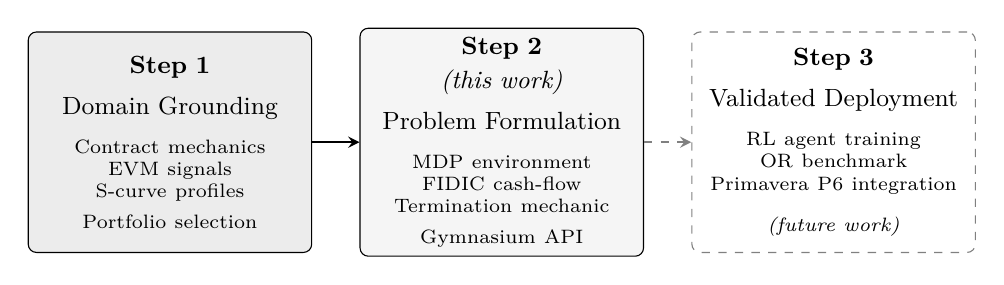
\begin{tikzpicture}[
    node distance  = 0cm,
    stepbox/.style = {rectangle, draw, rounded corners=3pt,
                      minimum width=3.6cm, minimum height=2.8cm,
                      align=center, font=\small, text width=3.2cm},
    arrow/.style   = {->, >=stealth, thick},
  ]

  \node[stepbox, fill=gray!15] (s1) at (0,0)
    {\textbf{Step 1}\\[4pt]
     Domain Grounding\\[6pt]
     \scriptsize
     Contract mechanics\\
     EVM signals\\
     S-curve profiles\\
     Portfolio selection};

  \node[stepbox, fill=gray!8, right=0.6cm of s1] (s2)
    {\textbf{Step 2}\\[1pt]
     \emph{(this work)}\\[4pt]
     Problem Formulation\\[6pt]
     \scriptsize
     MDP environment\\
     FIDIC cash-flow\\
     Termination mechanic\\
     Gymnasium API};

  \node[stepbox, draw=gray, dashed, right=0.6cm of s2] (s3)
    {\textbf{Step 3}\\[4pt]
     Validated Deployment\\[6pt]
     \scriptsize
     RL agent training\\
     OR benchmark\\
     Primavera~P6 integration\\[4pt]
     \emph{(future work)}};

  \draw[arrow]                    (s1) -- (s2);
  \draw[arrow, dashed, color=gray] (s2) -- (s3);

\end{tikzpicture}
\end{document}
